
\documentclass{beamer}

\mode<presentation> {
\usetheme{Warsaw}
\setbeamertemplate{footline}[page number] 

\setbeamertemplate{navigation symbols}{}
}

\usepackage[T2A]{fontenc}
\usepackage[cp1251]{inputenc}
\usepackage[english, russian]{babel}
\usepackage{amsmath}
\usepackage{amssymb,amsmath}
\usepackage{graphicx}

\def\mprp{\mbox{\tiny $\bot$}}
\def\mprl{\mbox{\tiny $\|$}}
\def\th{\mbox{th}}

\def\beq{\begin{eqnarray}}
\def\eeq{\end{eqnarray}}
\def\ee{\varepsilon}
\def\lm{\lambda}
\newcommand{\prp}[1]{#1_{\mbox{\tiny $\bot$}}}
\newcommand{\pprl}[1]{#1_{\mbox{\tiny $\|$}}}

\newcommand{\ii}{\mathrm{i}} 
\newcommand{\dd}{\mathrm{d}} 
\newcommand{\eee}{\mathrm{e}} 
\newcommand{\bs}{\boldsymbol} 


\def\D{\mathrm{d}} 


\usepackage{booktabs}
\usepackage{tkz-graph}
\GraphInit[vstyle = Shade]
\tikzset{
  LabelStyle/.style = { rectangle, rounded corners, draw,
                        minimum width = 2em, fill = yellow!50,
                        text = red, font = \bfseries },
  VertexStyle/.append style = { inner sep=5pt,
                                font = \normalsize\bfseries},
  EdgeStyle/.append style = {->, bend left} }
\usetikzlibrary {positioning}
\definecolor {processblue}{cmyk}{0.96,0,0,0}
%----------------------------------------------------------------------------------------
%	TITLE PAGE
%----------------------------------------------------------------------------------------

\title{Комптоноподобные процессы рассеяния во внешней активной среде}

\author{Денис Михайлович Шленев}
\institute[Ярославский государственный университет им. П.Г. Демидова] 
{
Ярославский государственный университет им. П.Г. Демидова\\ 
\medskip
}
\date{30 сентября 2021 г.} 


\begin{document}

\begin{frame}
\titlepage

\begin{center}

\vspace*{-4mm} 

{\small {Научный руководитель: д.ф.-м.н, профессор Д.А. Румянцев}} 

\vspace*{4mm} 

{\small Диссертация на соискание ученой степени 

кандидата физико-математических наук}
 

\end{center}
\end{frame}


\begin{frame}
\frametitle{Содержание}
\begin{itemize}

\item Введение

\item Обобщённые комптоноподобные процессы
рассеяния в замагниченной среде с учётом
возможного резонанса на виртуальном электроне

\item Резонансные квантовые процессы во внешней активной среде

\item Процесс расщепления фотона в сильном
магнитном поле и плазме с учётом влияния позитрония 

\item Заключение

\end{itemize}
 
\end{frame}

%%%%%%%%%%%%%%%%%%%%%%%%%%%%%%%%%%%%%%%%%%%%%%%%%%%%%%%%%%%%%%%%%%%%%%%%%%%%%%%%%%%%%%% 
\begin{frame}{Введение}

\begin{center}
Две составляющие внешней активной среды:
\end{center}
\begin{itemize}
\item Магнитное поле

Характерный масштаб: $B_e = \frac{m^2 c^3}{e\hbar} \simeq 4.41\cdot 10^{13}$ Гс

$B\sim 10^{12}$ Гс -- радиопульсары

$B\sim 10^{14}-10^{15}$ Гс -- магнитары

\item Относительно плотная плазма

В окрестности магнитаров и радиопульсаров концентрация $e^{+} e^{-}$-плазмы
порядка
$$n_{GJ} \simeq 3\cdot 10^{13} \text{см}^{-3} \left (\frac{B}{100 B_e} \right ) \left (\frac{10 \text{ сек}}{P} \right )\, .$$
$P=2\pi/\Omega$ - период обращения нейтронной звезды.


\end{itemize}
\end{frame}
%%%%%%%%%%%%%%%%%%%%%%%%%%%%%%%%%%%%%%%%%%%%%%%%%%%%%%%%%%%%%%%%%%%%%%%%%%%%%%%%%%%%%%%%
\begin{frame}{Введение}
\begin{center}
Две составляющие влияния внешней активной среды:
\end{center}
\begin{itemize}
\item \alert{Модификация амплитуд процессов}

Становятся возможными резонансы на виртуальном фермионе.

\begin{itemize}
\item Комптоновское рассеяние $e\gamma\to e \gamma$

\item Фотонейтринный процесс $e\gamma\to e\nu\bar\nu$ 
\end{itemize}
\item \alert{Модификация дисперсионных свойств частиц}

Новый канал расщепления фотона, $\gamma\to\gamma\gamma$
\end{itemize}
\end{frame}
%%%%%%%%%%%%%%%%%%%%%%%%%%%%%%%%%%%%%%%%%%%%%%%%%%%%%%%%%%%%%%%%%%%%%%%%%%%%%%%%%%%%%%
%                                                                                        %
%%%			Pt. 1							       %%%
%                                                                                        %
%%%%%%%%%%%%%%%%%%%%%%%%%%%%%%%%%%%%%%%%%%%%%%%%%%%%%%%%%%%%%%%%%%%%%%%%%%%%%%%%%%%%%%%%%%
\begin{frame}{Обобщённые комптоноподобные процессы рассеяния...}
\begin{center}
Краткий обзор литературы по одно- и двухвершинным процессам
\end{center}

\begin{itemize}
\item 1966 -- А.А. Соколов, И.М. Тернов -- процесс $e\to e \gamma$ в постоянном однородном магнитном поле
\item 1979 -- H. Herold -- процесс $e\gamma\to e \gamma$ в магнитном поле
\item 1999 -- М.Ю. Боровков, А.В. Кузнецов, Н.В.  Михеев -- двухвершинные 
амплитуды вида $jf\to j^{\, \prime} f^{\prime}$ в магнитном поле
\item 2015 -- А.В. Кузнецов, Д.А. Румянцев, {\bf Д.М. Шленев} -- обобщение предыдущего результата 
в магнитном поле на случай замагниченной плазмы в отсутствие резонанса
\item 2016 -- A.A. Mushtukov, D.I. Nagirner, J. Poutanen -- резонанс в процессе 
$e\gamma\to e \gamma$ в магнитном поле радиопульсара
\end{itemize}
\end{frame}
%%%%%%%%%%%%%%%%%%%%%%%%%%%%%%%%%%%%%%%%%%%%%%%%%%%%%%%%%%%%%%%%%%%%%%%%%%%%%%%%%%%%%%%%%
\begin{frame}{Обобщённые комптоноподобные процессы рассеяния...}
\begin{center}
Лагранжиан взаимодействия $jf\to j^{\, \prime} f^{\prime}$

${\cal L}(x) \, = \, \sum \limits_{k} g_k 
[\bar {\Psi}_f (X) \Gamma_k \Psi_f(X)]\, J_k(X),$
$k=S, P, V, A$

Диаграммы Фейнмана для процесса $jf\to j^{\, \prime} f^{\prime}$
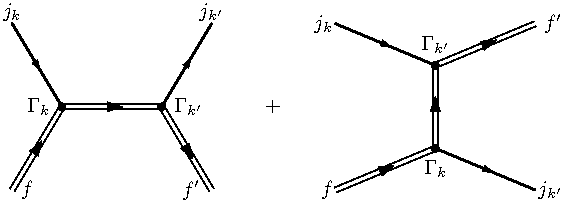
\includegraphics[width=10cm]{fig1_1-eps-converted-to.pdf}
\end{center}
${\cal S}^{s^{\, \prime} s}_{k^{\, \prime} k} = - g_k g_{k'}\int \dd^4 X \dd^4 Y \langle J_k (X) J_{k'} (Y) \rangle 
\left [\bar \Psi^{s'}_{p',\ell'}(Y) \Gamma_{k'} 
\hat S(Y,X) 
\Gamma_k \Psi^{s}_{p,\ell}(X) \right ] + (J_k, \Gamma_k \leftrightarrow J_{k'}, \Gamma_{k'})\, .$
\end{frame}
%%%%%%%%%%%%%%%%%%%%%%%%%%%%%%%%%%%%%%%%%%%%%%%%%%%%%%%%%%%%%%%%%%%%%%%%%%%%%%
\begin{frame}{Обобщённые комптоноподобные процессы рассеяния...}
\begin{center}

Возможны две ситуации:
\begin{itemize}
\item
При условии, что уровень Ландау виртуального фермиона меньше или равен
уровням Ландау начального и конечного фермиона, реальная часть знаменателя пропагатора
не обращается в ноль, что говорит о невозможности резонанса на виртуальном фермионе.
\vspace*{3mm}

\alert{Осн. результаты:} вычислены амплитуды рассеяния для всевозможных комбинаций вершин.

\vspace*{3mm}

\item Если уровень Ландау виртуального фермиона больше, чем 
у начального и конечного фермиона, то реальная часть знаменателя пропагатора может обращаться в ноль, 
т.е. виртуальный фермион становится реальным с определённым законом дисперсии и 
имеет место резонанс на виртуальном фермионе.

\end{itemize}
\end{center}
\end{frame}
%%%%%%%%%%%%%%%%%%%%%%%%%%%%%%%%%%%%%%%%%%%%%%%%%%%%%%%%%%%%%%%%%%%%%%%%%%%%%%%%
\begin{frame}{Обобщённые комптоноподобные процессы рассеяния...}
\begin{center}
Факторизация квадрата амплитуды в области резонанса
$${\cal M}^{s^{\, \prime} s}_{k^{\, \prime} k}\simeq \sum\limits_{n=0}^{\infty}
\sum\limits_{s''=\pm 1} \int \dd X_1 \dd Y_1 
\frac{(...)}{P^2_{\mprl}-M_n^2-\ii P_0\Gamma_n^{s''}/2}+...$$
%
$M_n = \sqrt{m^2+2eBn}$, $P_{\alpha} = (p+q)_{\alpha}$, 
$P^2_{\mprl} = P_0^2-P_z^2$, 

$\Gamma_n^{s''}$ -- полная ширина поглощения фермиона
%
$$|{\cal M}^{s^{\, \prime} s}_{k^{\, \prime} k}|^2 \simeq  \sum\limits_{s''=\pm 1} \sum\limits_{n=0}^{\infty} \;  
\frac{\pi}{P_0 \; \Gamma_n^{s''}} \; \alert{\delta (P^{2}_{\mprl} - M_n^2)}
\left |{\cal M}^{s' s''}_{(n,s'') \to j'f'}\right |^2 \left |{\cal M}^{s'' s}_{jf \to (n, s'')}\right |^2$$ 

\alert{Вычислены} одновершинные амплитуды 

${\cal M}^{s'' s}_{jf \to (n, s'')}$ и ${\cal M}^{s' s''}_{(n,s'') \to j'f'}$ перехода
из начального состояния $jf$ в промежуточное и из промежуточного в конечное состояние $j'f'$.
\end{center}
\end{frame}
%%%%%%%%%%%%%%%%%%%%%%%%%%%%%%%%%%%%%%%%%%%%%%%%%%%%%%%%%%%%%%%%%%%%%%%%%%%%%%%%
\begin{frame}{Обобщённые комптоноподобные процессы рассеяния...}

\begin{center}
Основные публикации по результатам Главы 1
\end{center}
% 
\begin{itemize}
%
\item
   A.~V.~Kuznetsov, D.~A.~Rumyantsev, and  D.~M.~Shlenev 
   Int.~J.~Mod.~Phys.~A {\bf 30}, 1550049 (2015)
% 
\item
   Д.~А.~Румянцев, Д.~М.~Шленев, А.~А.~Ярков

   ЖЭТФ {\bf 152}, 3 (9) (2017).
%
\item
  А~.В.~Кузнецов, Д.~А.~Румянцев, Д.~М.~Шленев

  Физика элементарных частиц и атомного ядра. 2017.
 
  Т. 48. Вып. 6. С. 980-983
\end{itemize}
\end{frame}
%%%%%%%%%%%%%%%%%%%%%%%%%%%%%%%%%%%%%%%%%%%%%%%%%%%%%%%%%%%%%%%%%%%%%%%%%%%%%%%%%%%%%%%%%%
%                                                                                        %
%%%			Pt. 2							       %%%
%                                                                                        %
%%%%%%%%%%%%%%%%%%%%%%%%%%%%%%%%%%%%%%%%%%%%%%%%%%%%%%%%%%%%%%%%%%%%%%%%%%%%%%%%%%%%%%%%%%
\begin{frame}{Резонансные квантовые процессы во внешней активной среде}
\begin{itemize}
\item Процесс \alert{$e\gamma\to e \gamma$} рассеяния фотона на электронах замагниченной среды 
для энергий начального фотона, близких к области резонанса.
\vspace*{3mm}

\alert{Условия:} магнитосфера радиопульсаров $B \sim 10^{12}$ Гс
\vspace*{3mm}

\item Процесс фоторождения нейтрино на электроне, \alert{$e\gamma\to e\nu\bar\nu$}
\vspace*{3mm}

\alert{Условия:} граница между внешней и внутренней корой магнитара

$B\sim 10^{14}-10^{16} \text{Гс}\gg B_e$, $T\sim 10^8-10^9 \text{К}\ll m$, $\rho\gtrsim 10^9 \text{г/см}^3$, %$\mu = 0$
\end{itemize}
\end{frame}
%%%%%%%%%%%%%%%%%%%%%%%%%%%%%%%%%%%%%%%%%%%%%%%%%%%%%%%%%%%%%%%%%%%%%%%%%%%%%%%%
\begin{frame}{Резонансные квантовые процессы во внешней активной среде}
\begin{center}
Обзор литературы по фотонейтринному процессу:
\end{center}
Первые работы
\begin{itemize}
\item 1961 -- В.И. Ритус
\item 1961 -- H.-Y. Chiu, R.C. Stabler
\end{itemize}
Вычисление нейтринной светимости за счёт процесса
\begin{itemize}
\item 1972 -- D.A. Dicus
\item 1989 -- N. Itoh et al.
\item 2000 -- В.В. Скобелев
\end{itemize}
С учётом дисперсионных свойств фотона в плазме, 
в отсутствие резонанса
\begin{itemize}
\item 2008 -- Д.А. Румянцев, М.В. Чистяков
\item 2012 -- А.В. Борисов, Б.К. Керимов, П.Е. Сизин
\item 2014 -- Н.В. Михеев, Д.А. Румянцев, М.В. Чистяков
\end{itemize}
\end{frame}
%%%%%%%%%%%%%%%%%%%%%%%%%%%%%%%%%%%%%%%%%%%%%%%%%%%%%%%%%%%%%%%%%%%%%%%%%%%%%%%%
\begin{frame}{Резонансные квантовые процессы во внешней активной среде}
\begin{center}

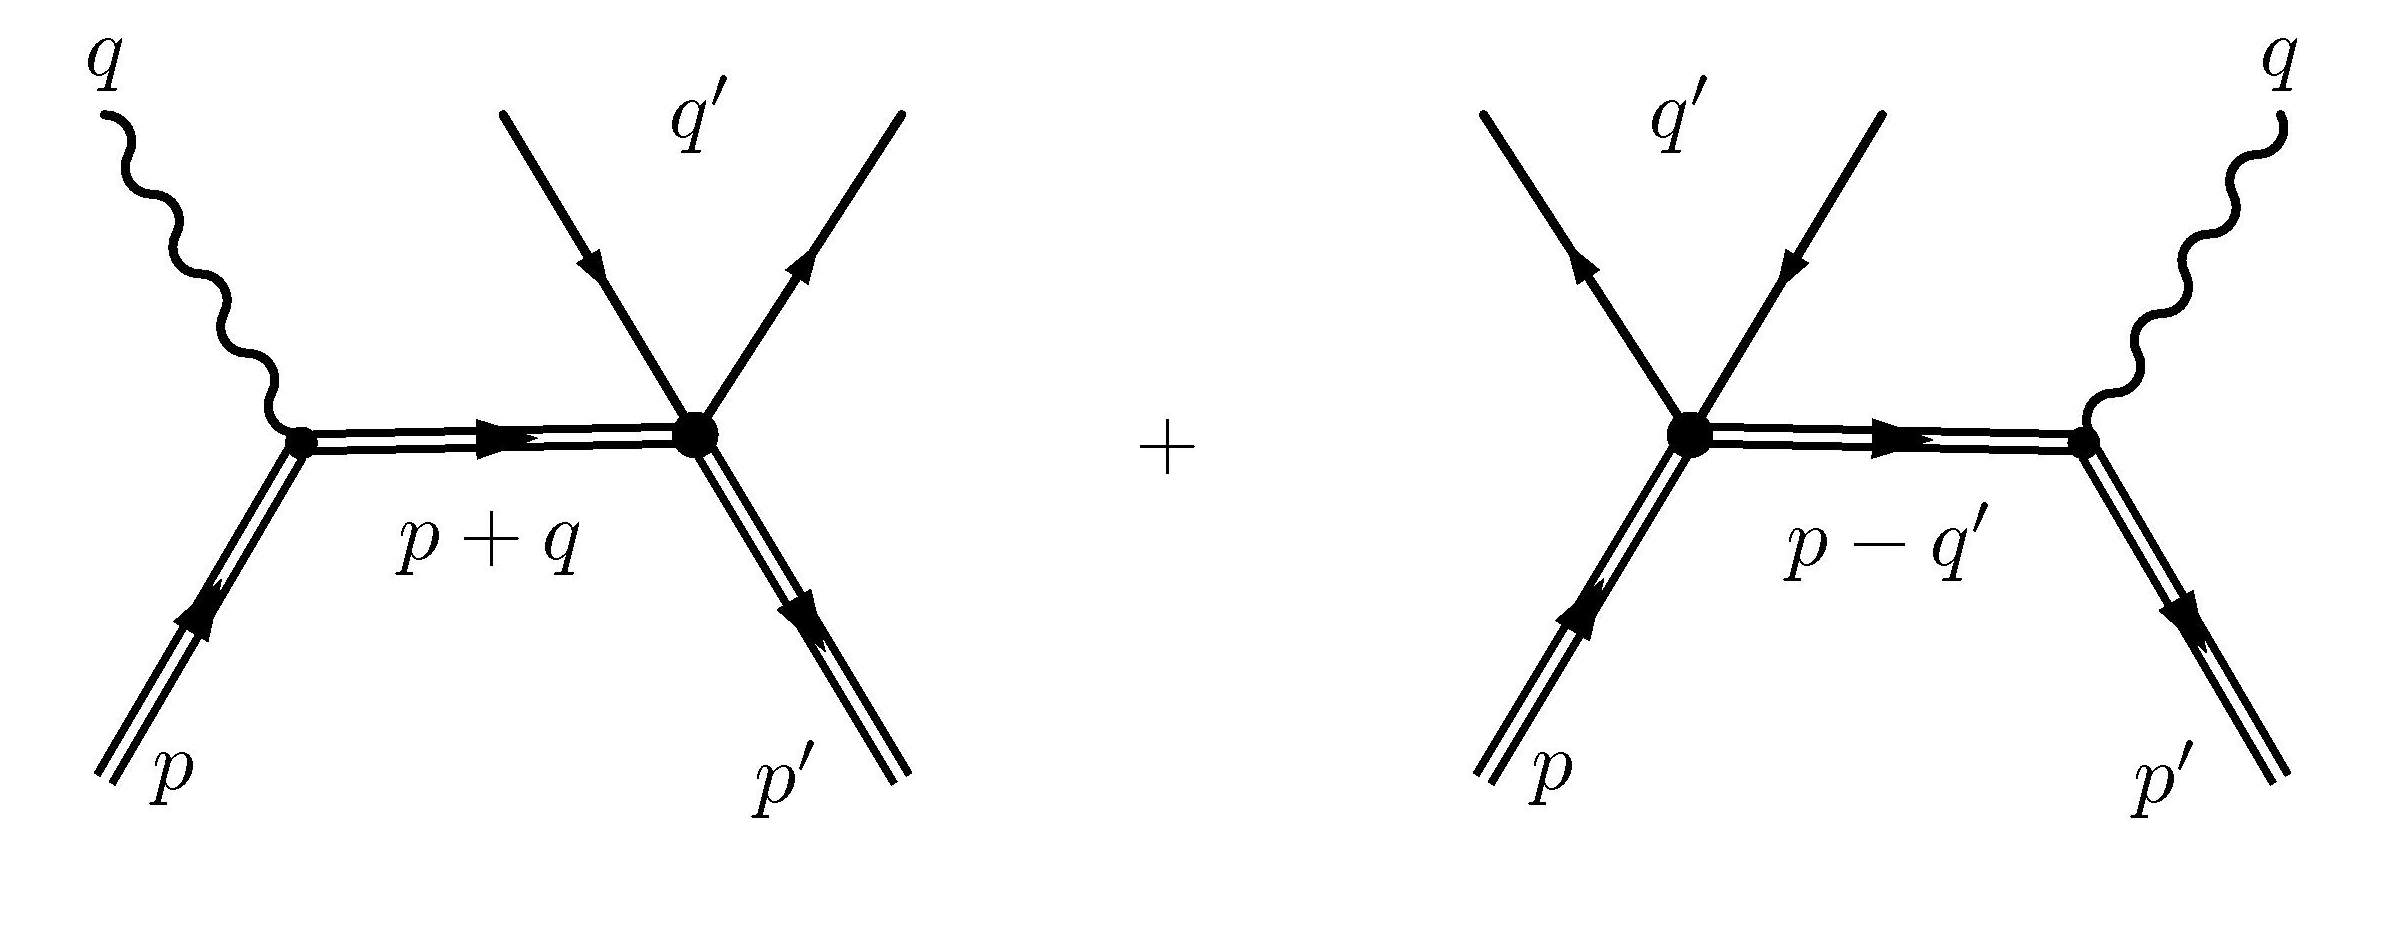
\includegraphics[scale=0.1]{fig00.jpg}

Нейтринная светимость за счёт процесса $e\gamma\to e\nu\bar\nu$ может быть представлена в виде:
%
\alert{$$Q_{\gamma e \to e \nu \bar \nu} = \sum\limits_{n=1}^{\infty}
\sum\limits_{\ell'=0}^{n-1}  
Q_{e_n \to e_{\ell'} \nu \bar \nu}  \, ,$$}
$Q_{e_n \to e_{\ell'} \nu \bar \nu}\,$-- нейтринная светимость за счёт процесса $e_n\to e_{\ell'}\nu\bar\nu$

(Д.Г. Яковлев и др. 2001)
\end{center}
\end{frame}
%%%%%%%%%%%%%%%%%%%%%%%%%%%%%%%%%%%%%%%%%%%%%%%%%%%%%%%%%%%%%%%%%%%%%%%%%%%%%%%%
\begin{frame}{Резонансные квантовые процессы во внешней активной среде}
\begin{center}
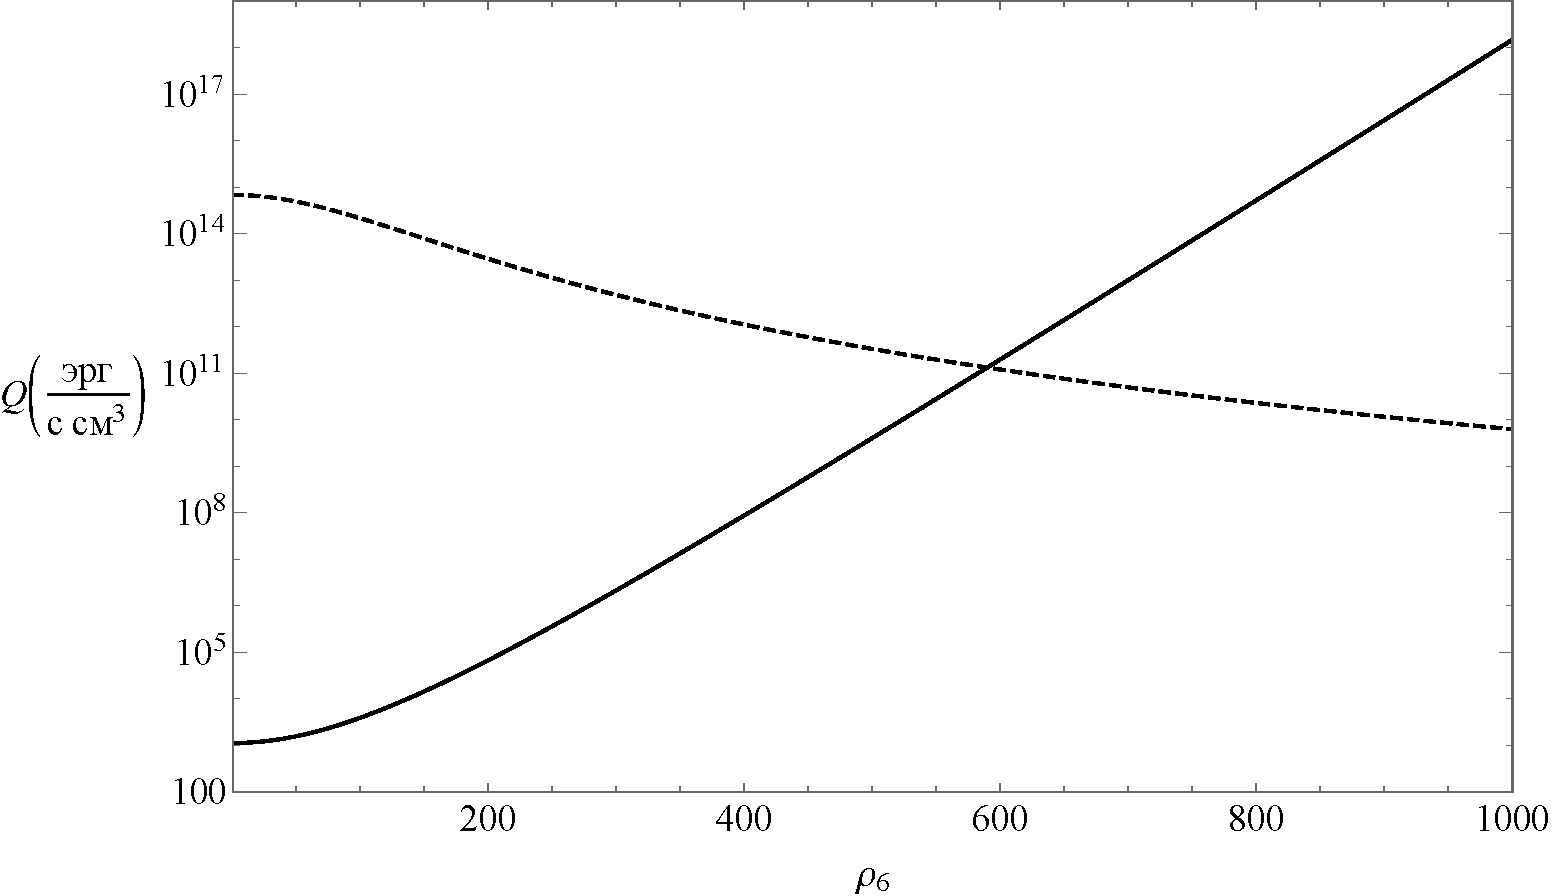
\includegraphics[scale=0.3]{Qsyn-Qpn 1.pdf}

Зависимость светимости фотонейтринного процесса от плотности плазмы ($\rho_6 = \rho /(10^6$ г/см$^3$)) для значений параметров 
$B=50 B_e$ и $T=10^9$~К. Сплошная линия соответствует светимости резонансного процесса, пунктирная -- без учёта резонанса

(Н.В. Михеев, Д.А. Румянцев, М.В. Чистяков 2014)
\end{center}
\end{frame}
%%%%%%%%%%%%%%%%%%%%%%%%%%%%%%%%%%%%%%%%%%%%%%%%%%%%%%%%%%%%%%%%%%%%%%%%%%%%%%%%%%%%%%%%%%
\begin{frame}{Резонансные квантовые процессы во внешней активной среде}

\begin{center}
Основные публикации по результатам Главы 2
\end{center}
% 
\begin{itemize}
%
\item
   A.~V.~Kuznetsov, D.~A.~Rumyantsev, and  D.~M.~Shlenev
 
   EPJ Web of Conferences 158, 05008 (2017)
% 
\item
   Д.~А.~Румянцев, Д.~М.~Шленев, А.~А.~Ярков

   ЖЭТФ {\bf 152}, 3 (9) (2017).
\end{itemize}
\end{frame}
%%%%%%%%%%%%%%%%%%%%%%%%%%%%%%%%%%%%%%%%%%%%%%%%%%%%%%%%%%%%%%%%%%%%%%%%%%%%%%%%%%%%%%%%%%
%                                                                                        %
%%%			Pt. 3							       %%%
%                                                                                        %
%%%%%%%%%%%%%%%%%%%%%%%%%%%%%%%%%%%%%%%%%%%%%%%%%%%%%%%%%%%%%%%%%%%%%%%%%%%%%%%%%%%%%%%%%%
\begin{frame}{Расщепление фотона в сильном магнитном поле...}
\begin{center}
Краткий обзор литературы по процессу $\gamma\to \gamma\gamma$

Магнитное поле без плазмы

\begin{itemize}
\item 1971 -- S.L. Adler

...

\item 1998 -- А.В.~Кузнецов, Н.В. Михеев, М.В. Чистяков
\item 2004 -- J.I. Weise

...

\item 2019 -- K. Hu, M.G. Baring, Z. Wadiasingh, A.K. Harding 
\end{itemize}

Электрон-позитронная плазма без магнитного поля

\begin{itemize}
\item 1974 -- D.B. Melrose
\item 1986 -- A.E. Shabad
\end{itemize}

Замагниченная электрон-позитронная плазма

\begin{itemize}
\item 1998 -- T. Bulik
\item 2012 -- Д.А. Румянцев, Н.С. Стусь, М.В. Чистяков
\end{itemize}

\end{center}
\end{frame}
%%%%%%%%%%%%%%%%%%%%%%%%%%%%%%%%%%%%%%%%%%%%%%%%%%%%%%%%%%%%%%%%%%%%%%%%%%%%%%%%
\begin{frame}{Расщепление фотона в сильном магнитном поле...}
\begin{center}
\alert{Расщепление фотона в сильном магнитном поле с учётом позитрония}

\vspace{3mm}

Диаграммы Фейнмана для процесса $\gamma\to\gamma\gamma$ в сильном магнитном поле:

\vspace{3mm}

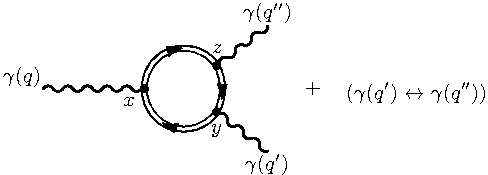
\includegraphics[scale=1]{fig3_1-eps-converted-to.pdf}

\end{center}
\end{frame}
%%%%%%%%%%%%%%%%%%%%%%%%%%%%%%%%%%%%%%%%%%%%%%%%%%%%%%%%%%%%%%%%%%%%%%%%%%%%%%%%%%%%%%%%%%
\begin{frame}{Расщепление фотона в сильном магнитном поле...}
\begin{center}
\alert{Дисперсия фотона в сильном магнитном поле с учётом влияния позитрония.}

\vspace*{2mm}

Можно ввести два поляризационных состояния фотона:
$$\varepsilon_\alpha^{(1)}(q) = \frac{(q \varphi)_\alpha}{\sqrt{q_{\mprp}^2}},
\qquad
\varepsilon_\alpha^{(2)}(q) = \frac{(q \tilde \varphi)_\alpha}
{\sqrt{q_{\mprl}^2}}.$$

Символы 1 и 2 соответствуют $\mprl$ и $\mprp$ поляризациям в работе (Adler 1971), X- и O-модам в работе (Mushtukov et al. 2016)

и E- и O-модам в работе (Thompson et al. 1995).

\vspace*{2mm}

\alert{Для фотона моды 2 возникает область с $q^2 > 0$.}
\end{center}
\end{frame}
%%%%%%%%%%%%%%%%%%%%%%%%%%%%%%%%%%%%%%%%%%%%%%%%%%%%%%%%%%%%%%%%%%%%%%%%%%%%%%%%
\begin{frame}{Расщепление фотона в сильном магнитном поле...}
\begin{center}
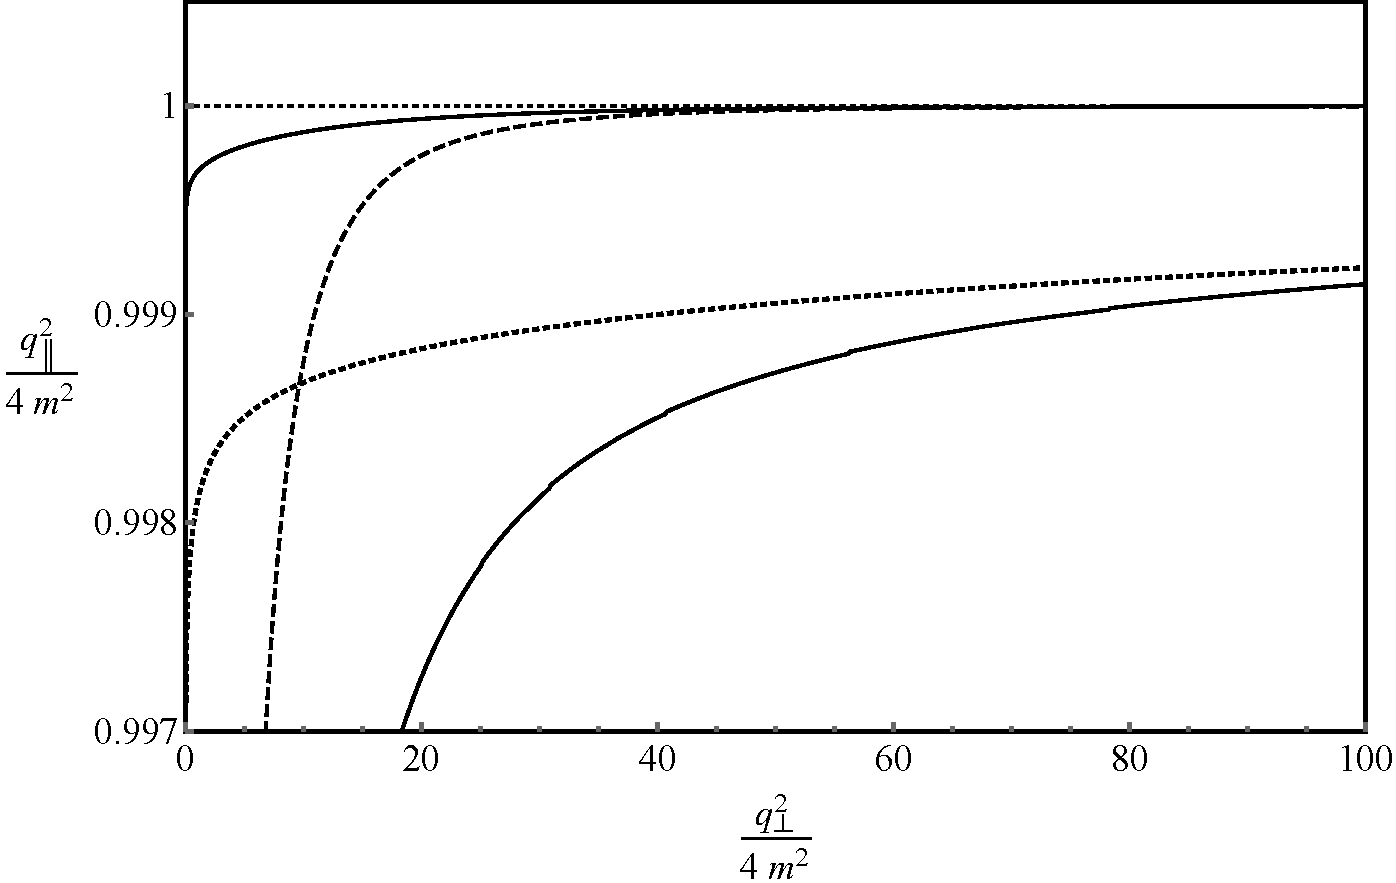
\includegraphics[scale=0.35]{Disp200.pdf}

Закон дисперсии фотона 2 моды для $B = 200B_e$, $\theta = \pi/2$.

Пунктирная кривая -  спектральная линия фотона без учёта вклада позитрония,

точечная кривая - спектральная линия позитрония.
\end{center}
\end{frame}
%%%%%%%%%%%%%%%%%%%%%%%%%%%%%%%%%%%%%%%%%%%%%%%%%%%%%%%%%%%%%%%%%%%%%%%%%%%%%%%%%%%%%%%%%%
%\begin{frame}{Расщепление фотона в сильном магнитном поле...}
%\begin{center}
%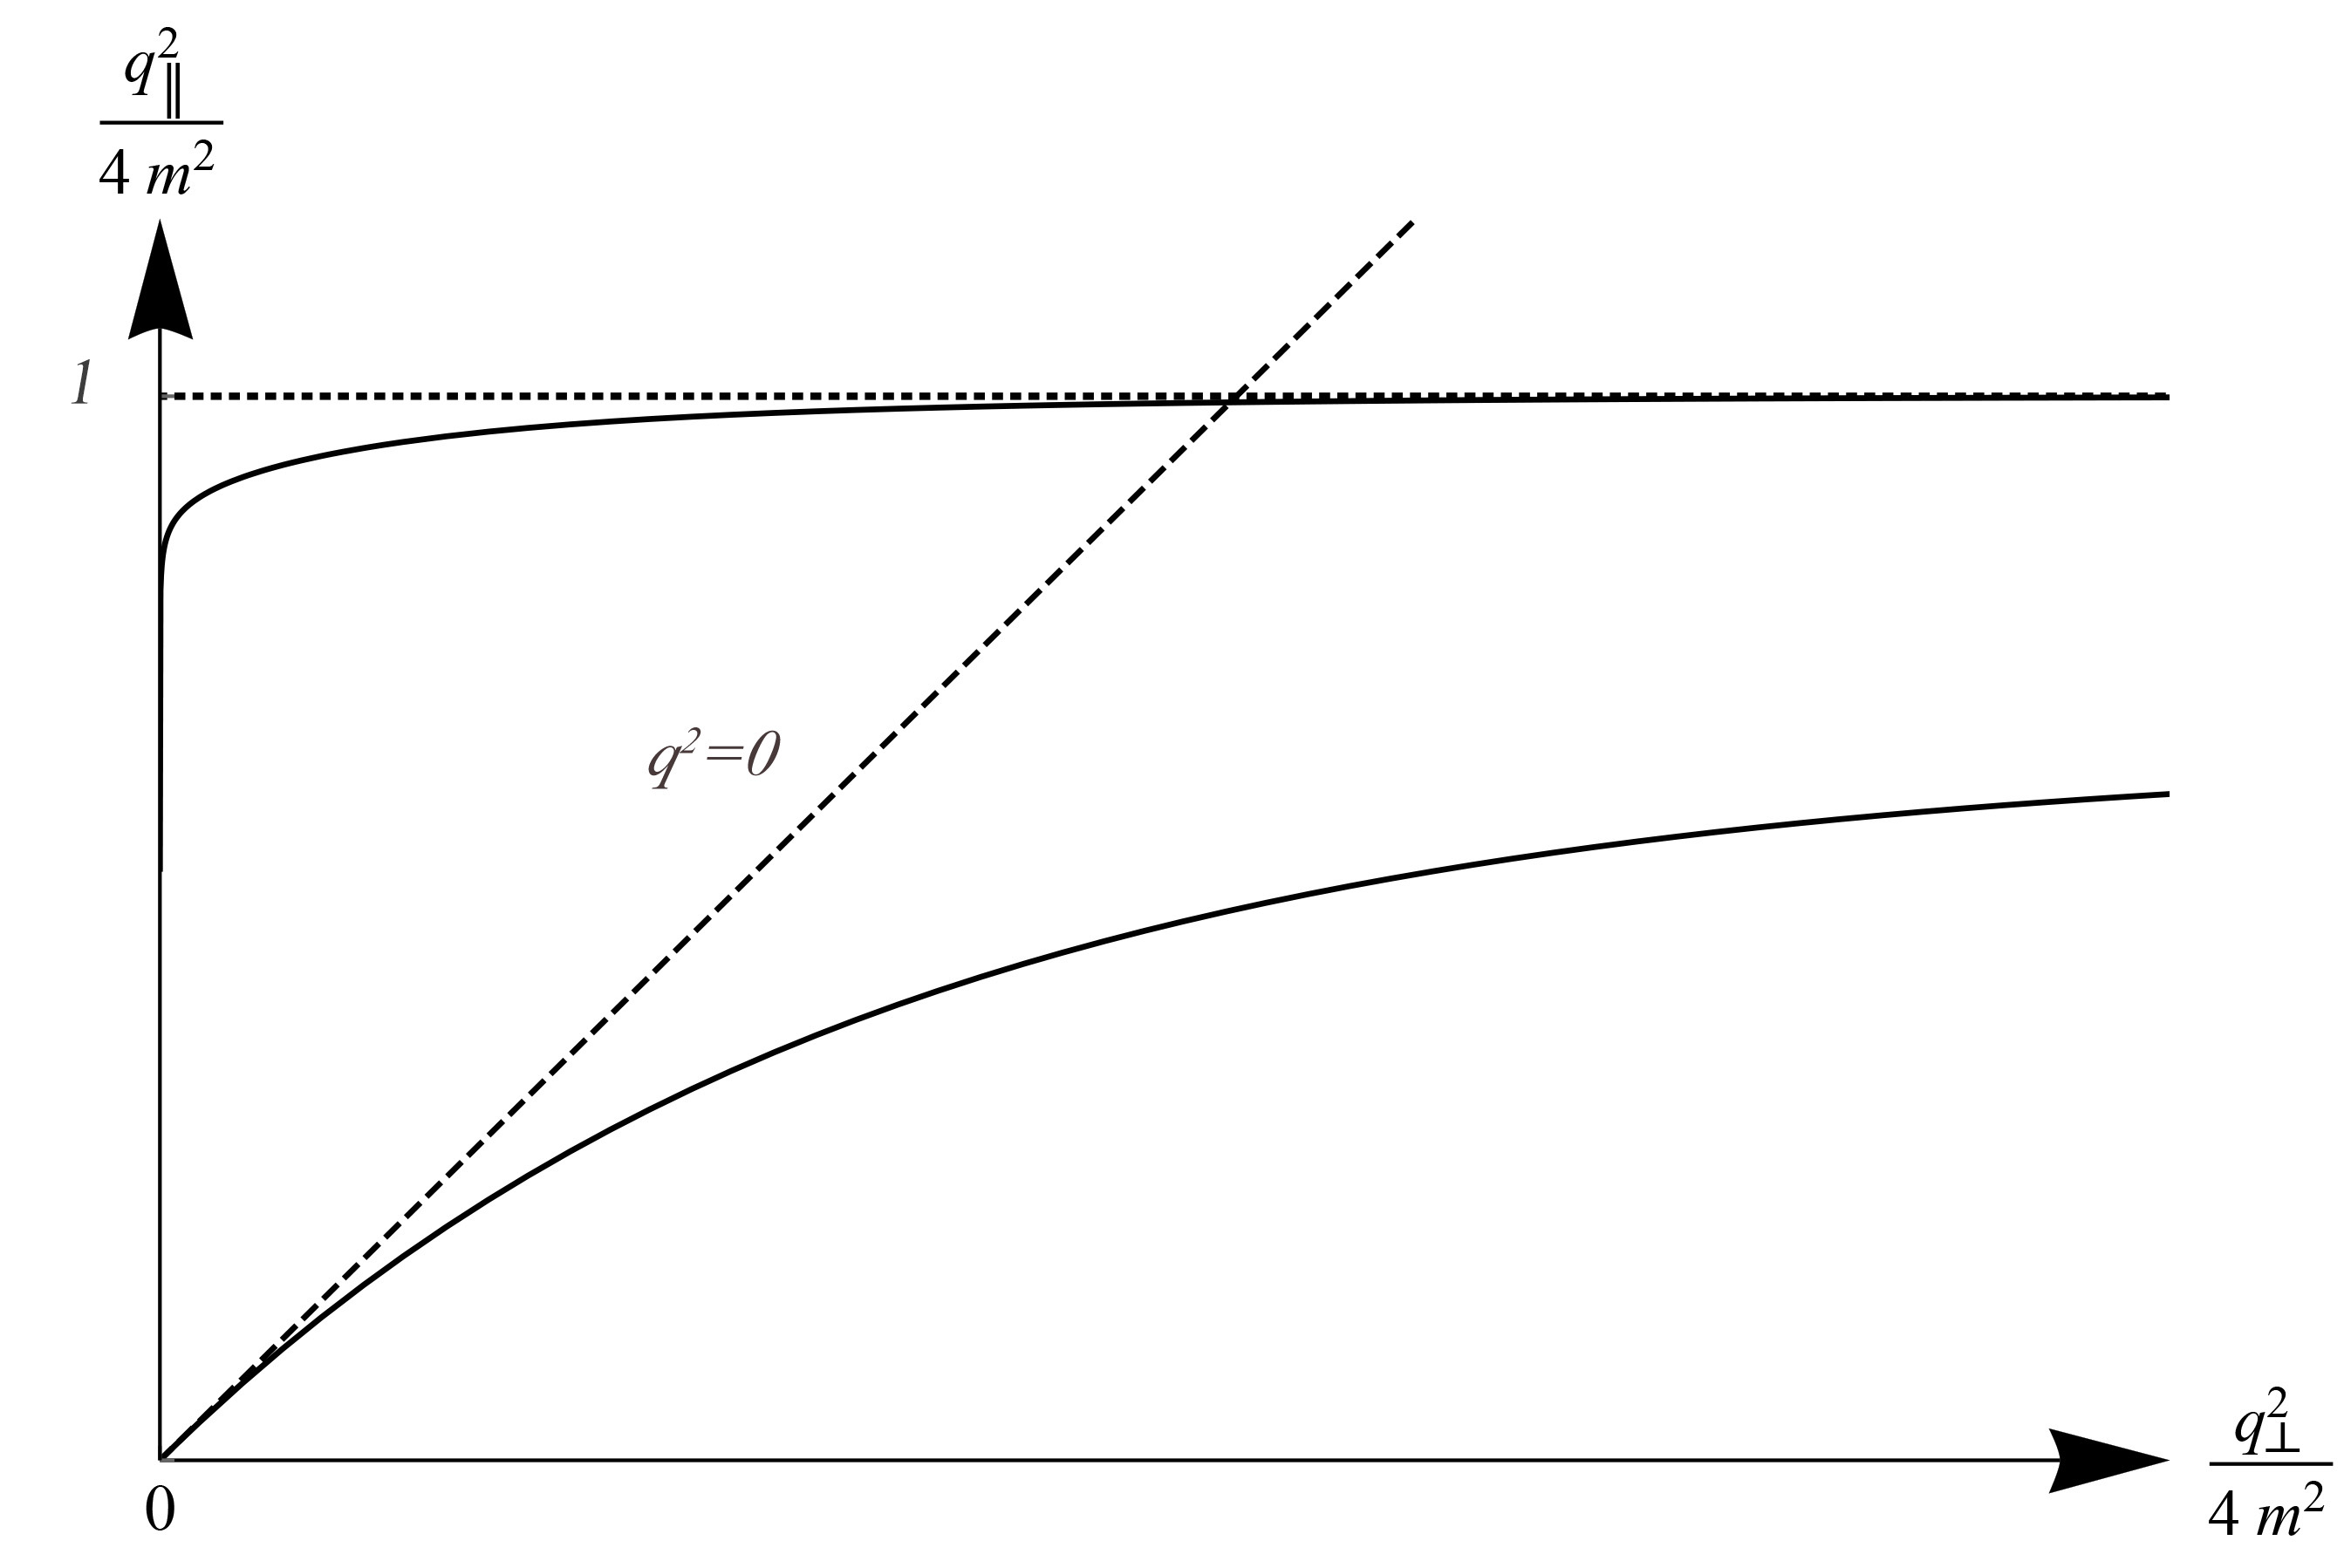
\includegraphics[scale=0.45]{SelRules.jpg}
%\end{center}
%\end{frame}
%%%%%%%%%%%%%%%%%%%%%%%%%%%%%%%%%%%%%%%%%%%%%%%%%%%%%%%%%%%%%%%%%%%%%%%%%%%%%%%%
\begin{frame}{Расщепление фотона в сильном магнитном поле...}
\begin{center}
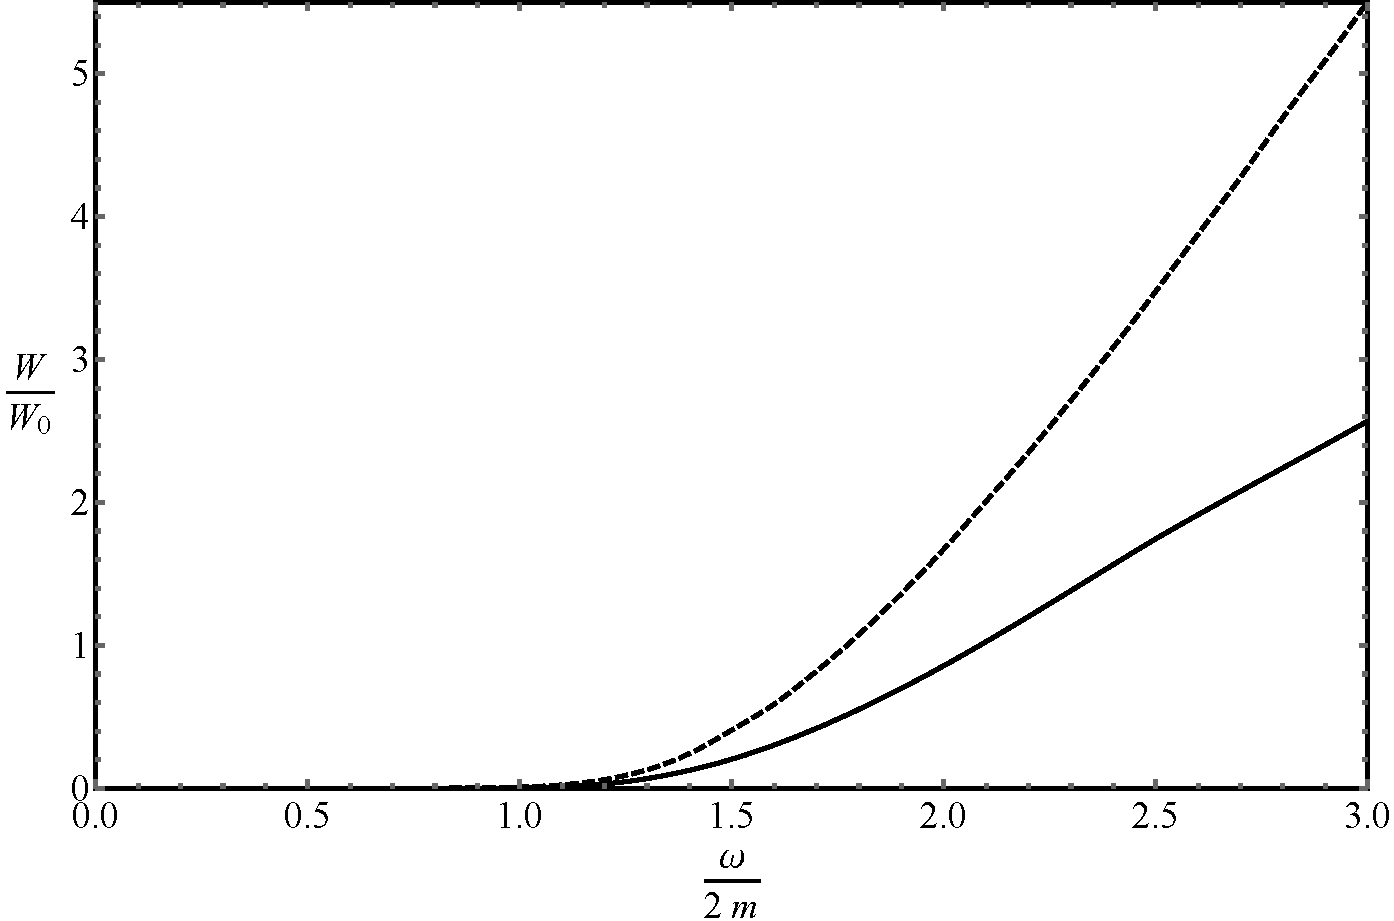
\includegraphics[scale=0.28]{112.pdf}

Вероятность процесса расщепления фотона в канале $\gamma_1 \to\gamma_1 \gamma_2$ в сильном 
магнитном поле ($B=200 B_e$) с учётом влияния позитрония.

Пунктирная линия - вероятность реакции без учёта вклада позитрония.

\end{center}
\end{frame}
%%%%%%%%%%%%%%%%%%%%%%%%%%%%%%%%%%%%%%%%%%%%%%%%%%%%%%%%%%%%%%%%%%%%%%%%%%%%%%
\begin{frame}{Расщепление фотона в сильном магнитном поле...}
\begin{center}
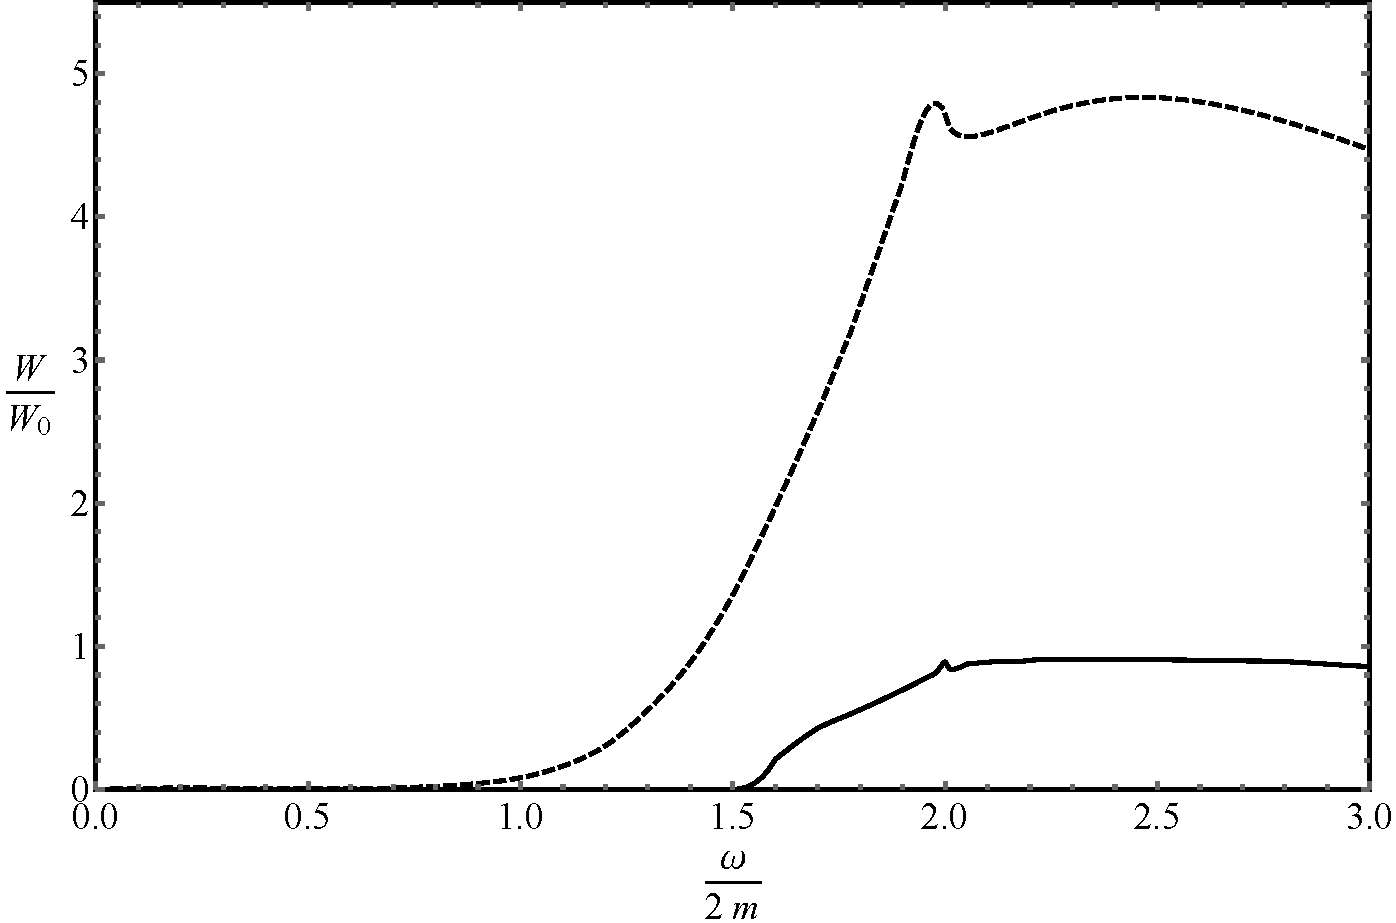
\includegraphics[scale=0.31]{122.pdf}

Вероятность процесса расщепления фотона в канале $\gamma_1 \to\gamma_2 \gamma_2$ в сильном 
магнитном поле ($B=200 B_e$) с учётом влияния позитрония.

Пунктирная линия - вероятность реакции без учёта вклада позитрония.
\end{center}
\end{frame}
%%%%%%%%%%%%%%%%%%%%%%%%%%%%%%%%%%%%%%%%%%%%%%%%%%%%%%%%%%%%%%%%%%%%%%%%%%%%%%
\begin{frame}{Расщепление фотона в сильном магнитном поле...}
\begin{center}
Вероятность процесса расщепления фотона в канале $\gamma_2 \to\gamma_1 \gamma_1$ в сильном 
магнитном поле с учётом влияния позитрония:

$$W_{2 \to 11} = 
\frac{\alpha^3}{8\pi^2}\, Z_2\,  H^2\left(\frac{q^2_{\mprl}}{4m^2}\right)
\frac{q_{\mprp}^2}{\omega} \, {\cal F}\left
(\sqrt{\frac{q_{\mprl}^2}{q_{\mprp}^2}} \right) \, \Theta (q^2)\, ,$$
%
$$H(z)=\frac{1}{\sqrt{z(1 - z)}} \, \arctg \sqrt{\frac{z}{1 - z}} - 1 \, ,$$
%
$$Z_2^{-1} = 1 - \frac{\partial\varkappa^{(2)}}{\partial q_{\mprl}^2},$$ $\varkappa^{(2)}$ -- собственное значение поляризационного оператора 
для фотона моды 2,
%
$${\cal F}(z) \, = \, 2 \ln{z} \, - \, 1 \, + \, z^{-2} \, .$$

\end{center}
\end{frame}
%%%%%%%%%%%%%%%%%%%%%%%%%%%%%%%%%%%%%%%%%%%%%%%%%%%%%%%%%%%%%%%%%%%%%%%%%%%%%%
\begin{frame}{Расщепление фотона в сильном магнитном поле...}
\begin{center}
Коэффициент поглощения фотона в канале $\gamma_2 \to\gamma_1 \gamma_1$ в сильном 
магнитном поле с учётом влияния позитрония при $B = 200 B_e$:

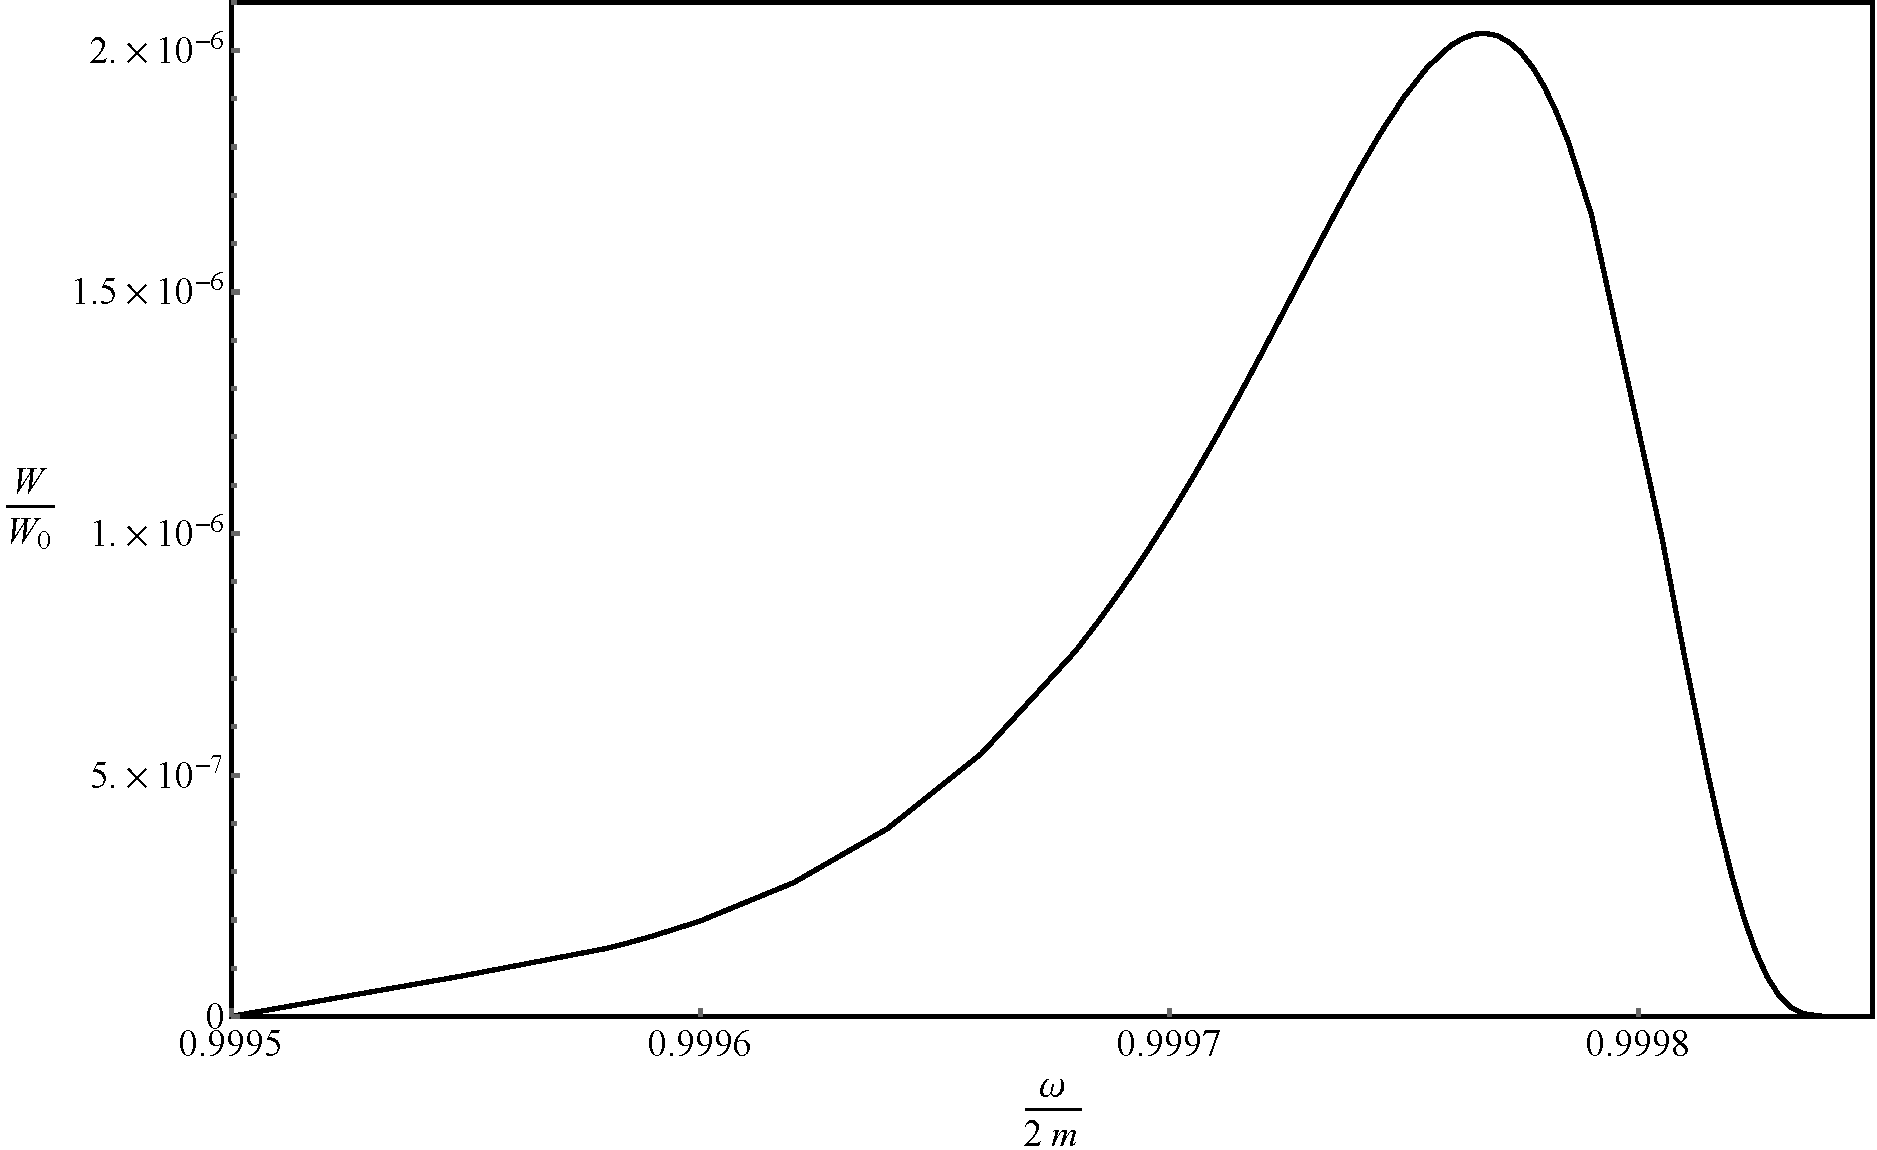
\includegraphics[scale=0.28]{211pos.pdf}

\end{center}
\end{frame}
%%%%%%%%%%%%%%%%%%%%%%%%%%%%%%%%%%%%%%%%%%%%%%%%%%%%%%%%%%%%%%%%%%%%%%%%%%%%%%%%
\begin{frame}{Расщепление фотона в сильном магнитном поле...}

\begin{center}
Основные публикации по результатам Главы 3
\end{center}
% 
\begin{itemize}
%
\item
  M.~V.~Chistyakov, D.~A.~Rumyantsev, and D.~M.~Shlenev
 
  EPJ Web of Conferences 19. 2016. P. 04017.

\item R.~A.~Anikin, M.~V.~Chistyakov, D.~A.~Rumyantsev, D.~M.~Shlenev,
 EPJ Web Conf. 2018. Vol. 191. P. 08011.
\end{itemize}
\end{frame}

%%%%%%%%%%%%%%%%%%%%%%%%%%%%%%%%%%%%%%%%%%%%%%%%%%%%%%%%%%%%%%%%%%%%%%%%%%%%%%
\begin{frame}{Заключение}
\begin{itemize}

\item Впервые исследованы возможные резонансные эффекты в древесных двухвершинных 
амплитудах для переходов $jf\to j^{\,\prime} f^{\,\prime}$ в постоянном однородном 
магнитном поле и в присутствии замагниченной плазмы, где  $f$ и $f'$ - начальный и 
конечный фермионы, находящиеся на произвольных уровнях Ландау, $j$ и $j'$ - 
обобщенные токи скалярного, псевдоскалярного, векторного или  аксиального 
типов. Показано, что в области резонанса амплитуды реакции $jf\to j^{\,\prime} f^{\,\prime}$ 
однозначно выражаются через амплитуды процессов $jf\to \tilde f$ и  
$\tilde f\to j^{\,\prime} f^{\,\prime}$, содержащих промежуточное состояние $\tilde f$.


\end{itemize}
\end{frame}
%%%%%%%%%%%%%%%%%%%%%%%%%%%%%%%%%%%%%%%%%%%%%%%%%%%%%%%%%%%%%%%%%%%%%%%%%%%%%%%


\begin{frame}{Заключение}
\begin{itemize}
\item Впервые вычислена нейтринная 
излучательная способность, обусловленная процессом 
$\gamma e\to e\nu\bar\nu$ в холодной  замагниченной 
плазме с учетом резонанса на виртуальном электроне, 
занимающем произвольный уровень Ландау $n$. 
Впервые получен коэффициент поглощения фотона в процессе
резонансного рассеяния $\gamma e\to\gamma e$ 
в присутствии замагниченной плазмы, результат 
представлен в простой аналитической форме, 
удобной для дальнейшего использования при 
решении задачи переноса излучения. Показано, что использование  
$\delta$-функциональной аппроксимации резонансных пиков 
в области резонансов хорошо согласуется  с 
соответствующими в литературе результатами, 
полученными громоздкими численными расчетами.

\end{itemize}
\end{frame}
%%%%%%%%%%%%%%%%%%%%%%%%%%%%%%%%%%%%%%%%%%%%%%%%%%%%%%%%%%%%%%%%%%%%%%%%%%%%%%%


\begin{frame}{Заключение}
\begin{itemize}
\item Найдены правила отбора по поляризациям для 
процесса расщепления фотона $\gamma\to\gamma\gamma$ 
в холодной почти вырожденной плазме и в сильном магнитном поле с 
учётом вклада позитрония.
Для разрешённых каналов расщепления фотона вычислены 
парциальные вероятности процесса с учётом влияния 
замагниченной холодной плазмы и позитрония 
в дисперсию и перенормировку волновых 
функций фотонов. 
Полученные результаты показывают, 
что вклады плазмы и позитрония, с одной стороны, существенным 
образом изменяют правила отбора по поляризациям по 
сравнению со случаем чистого магнитного поля. 
В частности, становится возможным новый канал 
расщепления $\gamma_2\to\gamma_1 \gamma_1$.
С другой стороны, вероятность расщепления по каналам 
$\gamma_1\to\gamma_1 \gamma_2$ 
и $\gamma_1\to\gamma_2 \gamma_2$ оказалась подавлена
по сравнению со случаем замагниченного вакуума.

\end{itemize}
\end{frame}
%%%%%%%%%%%%%%%%%%%%%%%%%%%%%%%%%%%%%%%%%%%%%%%%%%%%%%%%%%%%%%%%%%%%%%%%%%
\begin{frame}{Основные публикации}
% 
\begin{enumerate}
%
\item
   A.~V.~Kuznetsov, D.~A.~Rumyantsev, and  D.~M.~Shlenev 
   Int.~J.~Mod.~Phys.~A {\bf 30}, 1550049 (2015)
%
\item
  M.~V.~Chistyakov, D.~A.~Rumyantsev, and D.~M.~Shlenev
 
  EPJ Web of Conferences 19. 2016. P. 04017.
% 
\item
   Д.~А.~Румянцев, Д.~М.~Шленев, А.~А.~Ярков

   ЖЭТФ {\bf 152}, 3 (9) (2017).
%
\item
   A.~V.~Kuznetsov, D.~A.~Rumyantsev, and  D.~M.~Shlenev
 
   EPJ Web of Conferences 158, 05008 (2017)
%
\item
  А~.В.~Кузнецов, Д.~А.~Румянцев, Д.~М.~Шленев

  Физика элементарных частиц и атомного ядра. 2017. 
  Т. 48. Вып. 6. С. 980-983

\item R.~A.~Anikin, M.~V.~Chistyakov, D.~A.~Rumyantsev, D.~M.~Shlenev,
 EPJ Web Conf. 2018. Vol. 191. P. 08011.

\end{enumerate}
\end{frame}
%%%%%%%%%%%%%%%%%%%%%%%%%%%%%%%%%%%%%%%%%%%%%%%%%%%%%%%%%%%%%%%%%%%%%%%%%%%%%%%%%%%%%%%%%%
%                                                                                        %
%%%			Appendix						       %%%
%                                                                                        %
%%%%%%%%%%%%%%%%%%%%%%%%%%%%%%%%%%%%%%%%%%%%%%%%%%%%%%%%%%%%%%%%%%%%%%%%%%%%%%%%%%%%%%%%%%
\begin{frame}{Приложение}
\begin{center}
Реальная часть знаменателя пропагатора
$$(p+q)^2_{\mprl}-m^2-2eBn = 0;$$
$$p^2_{\mprl} = m^2+2eB\ell; \quad p^{\,\prime 2}_{\mprl} = m^2+2eB\ell^{\,\prime};$$
$$2(pq)_{\mprl}+q^2_{\mprl}=2eB(n-\ell);$$
$$\omega^2 > q_z^2; \quad E_{\ell}^2 > p_z^2;$$
$$E_{\ell}\, \omega - p_z q_z >0;$$
$$2(pq)_{\mprl}+q^2_{\mprl} > 0 \to n>\ell$$
\end{center}
\end{frame}
%%%%%%%%%%%%%%%%%%%%%%%%%%%%%%%%%%%%%%%%%%%%%%%%%%%%%%%%%%%%%%%%%%%%%%%%%%%%%%%%%%%%%%%%%%
\begin{frame}{Приложение}
\begin{center}
В формуле (1.77) квадрат знаменателя пропагатора был приближённо заменён следующим образом в (1.79):
$$\frac{1}{(P_{\mprl}^2-M_n^2+\ii \Im^{s''}_\Sigma)^2}  = \frac{\pi}{P_0\Gamma_n^{s''}}\delta(P_{\mprl}^2-M_n^2).$$
Правильная размерность при этом сохраняется.
\end{center}
\end{frame}
%%%%%%%%%%%%%%%%%%%%%%%%%%%%%%%%%%%%%%%%%%%%%%%%%%%%%%%%%%%%%%%%%%%%%%%%%%%%%%%%%%%%%%%%%%
\begin{frame}{Приложение}
\begin{center}
$$A_3^{(1,3)} = - \ii \, \frac{6 \Delta N \, \omega}{q_{\mprl}^2} \,$$
%
$$r^{(1,3)}_{\alpha} = \left [\mp \sqrt{q^4_{\mprp} + 
(6 \Delta N \, \omega)^2\, \frac{q^2}{q_{\mprl}^2}}  - q^2_{\mprp} \right ]\, 
b^{(1)}_{\alpha} - \ii \, \frac{6 \Delta N \, \omega}{q_{\mprl}^2} \,  b^{(3)}_{\alpha} +$$
$$+ \ii \,\frac{\Delta N \, k_z \, q^2_{\mprp}}{2\beta \, {\cal D} \, q^2_{\mprl}}\, 
\left [\pm \sqrt{q^4_{\mprp} + 
(6 \Delta N \, \omega)^2\, \frac{q^2}{q_{\mprl}^2}} + q^2_{\mprp} \right ]\; b^{(2)}_{\alpha} + 
O \left (\frac{1}{\beta^2} \right) \, ,$$
$$(r^{(3)})^2 = \left (\frac{6 \Delta N \, \omega}{q_{\mprl}^2}\right )^2 (b^{(3)})^2\, .$$
%
В пределе отсутствия плазмы $\Delta N = 0$:
$$\frac{r_{\alpha}^{(3)}}{\sqrt{(r^{(3)})^2}} = \frac{b_{\alpha}^{(3)}}{\sqrt{(b^{(3)})^2}}.$$
\end{center}
\end{frame}
%%%%%%%%%%%%%%%%%%%%%%%%%%%%%%%%%%%%%%%%%%%%%%%%%%%%%%%%%%%%%%%%%%%%%%%%%%%%%%%%%%%%%%%%%%
\begin{frame}{Приложение}
\begin{center}
Собственное значение поляризационного оператора для фотона моды 3:
$$\varkappa^{(3)} = \frac{\alpha}{3\pi} \, q^2 \, {\cal V} + \frac{\alpha}{6\pi} \, \left [ 
  \sqrt{q^4_{\mprp} + 
(6 \Delta N \, \omega)^2\, \frac{q^2}{q_{\mprl}^2}}  - q^2_{\mprp} \right ] \times$$ 
$$\times \left \{ 1 + \frac{3( \Delta N \, k_z)^2 \, q^2_{\mprp}}{2\beta \, 
{\cal D} \, q^2_{\mprl}}\, \left [ q^4_{\mprp} + 
(6\Delta N \, \omega)^2\, \frac{q^2}{q_{\mprl}^2} \right ]^{-1/2} \right \}
+ O \left (\frac{1}{\beta^2} \right)  \, ,$$
$${\cal V} = \ln{(B/B_e)} - 1.792 + \frac{3}{2} \, \int\limits_0^1 \dd x \, (1-x^2) \, 
\ln{\left [1- \frac{q^2}{4m^2} \, (1-x^2) \right ]} \, .$$
В холодной почти вырожденной плазме при выполнении условия:
$$\frac{\alpha \Delta N}{2 \pi m \sin{\theta}} = \frac{\alpha p_F}{\pi m \sin{\theta}} \ll 1$$
$$r_{\alpha}^{(3)}\sim q_{\alpha}$$
и может быть устранён калибровочным преобразованием.
\end{center}
\end{frame}
%%%%%%%%%%%%%%%%%%%%%%%%%%%%%%%%%%%%%%%%%%%%%%%%%%%%%%%%%%%%%%%%%%%%%%%%%%%%%%%%%%%%%%%%%%
\begin{frame}{Приложение}
\begin{center}
Энергия связи позитрония:
$$\varepsilon = \frac{\alpha^2 m}{4} \frac{1}{\nu^2}\, ,$$
$$\nu = \big [\ln (4.5 u) -2.44 \ln (\ln 0.15 u)) \big ]^{-1}\, ,$$
$$u = \frac{B / B_e}{\alpha^2} \frac{\exp (E_i (-\rho))}{\rho} \,,\quad E_i (-\xi) = \int\limits_{-\infty}^{-\xi} \frac{\exp t}{t} \dd t,$$
При $\rho < 1$
$$E_i (-\rho) = \gamma_E + \ln \rho + \sum\limits_{k=1}^{\infty} \frac{(-\rho)^k}{kk!} \, , \quad \gamma_E = 0.5772...$$
$$\lim_{\rho\to 0} \frac{\exp (E_i (-\rho))}{\rho} = \exp (\gamma_E)\, .$$
\end{center}
\end{frame}
%%%%%%%%%%%%%%%%%%%%%%%%%%%%%%%%%%%%%%%%%%%%%%%%%%%%%%%%%%%%%%%%%%%%%%%%%%%%%%%%%%%%%%%%%%
\begin{frame}{Приложение}
\begin{center}
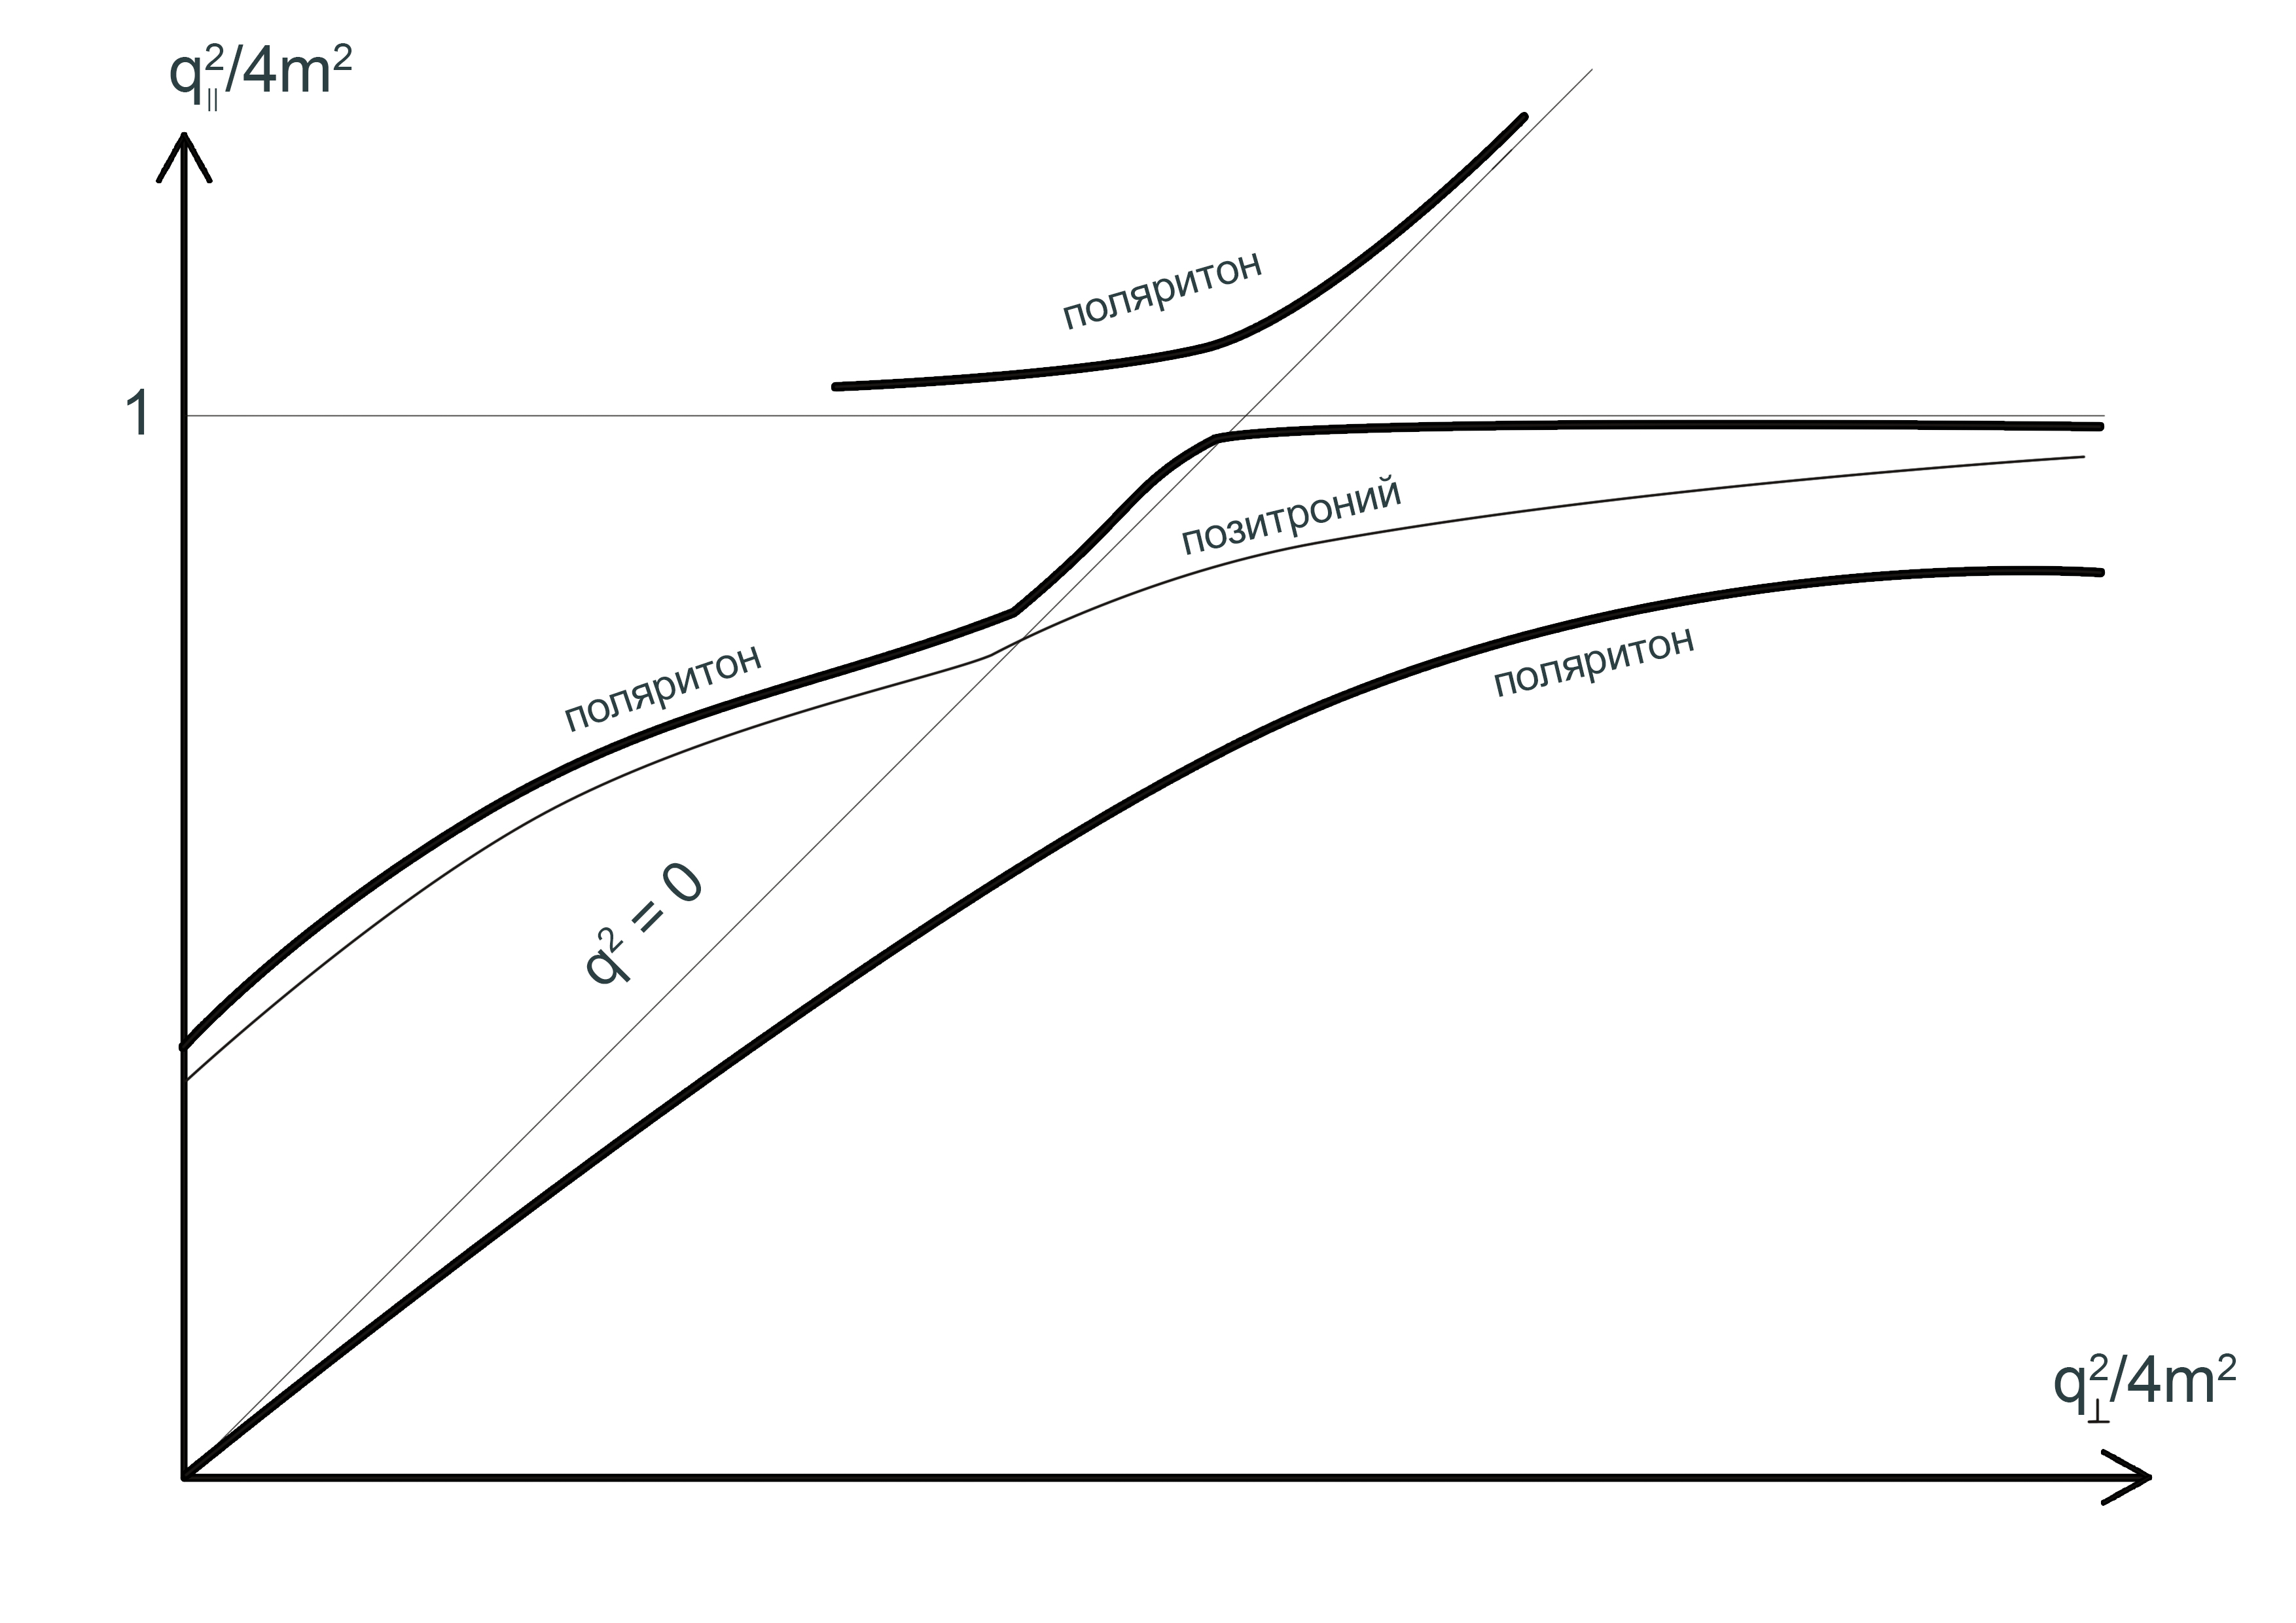
\includegraphics[width=10cm]{Disp.jpg}

Закон дисперсии для фотона моды 2 в сильном магнитном поле с учётом влияния позитрония
\end{center}
\end{frame}
%%%%%%%%%%%%%%%%%%%%%%%%%%%%%%%%%%%%%%%%%%%%%%%%%%%%%%%%%%%%%%%%%%%%%%%%%%%%%%%%%%%%%%%%%%
\end{document}
